
\og La croix de bûcheron\fg\ est un instrument permettant de
déterminer rapidement la hauteur d'un arbre. On l'utilise de la façon
suivante :
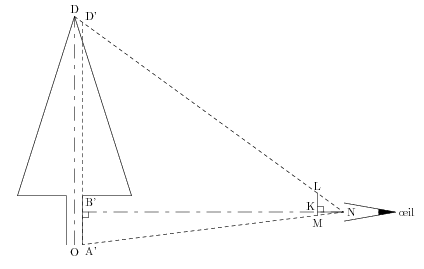
\includegraphics[scale=1]{TR-exo13.png} 
{\em La figure n'est pas en vraie grandeur.}\\
N'ayant pas besoin d'une précision importante sur la hauteur de
l'arbre, on suppose que la longueur $B'D'$ est la hauteur de l'arbre.
\\On donne les mesures suivantes : $KN=15$~cm; $LK=10$~cm; $KM=1,5$~cm
et $B'N=27$~m.
\\Détermine alors \og la hauteur de l'arbre\fg\ $B'D'$.
 